\section{Results}

    This section introduces all the results provide by Alloy through the predicates above. `Check' allows the analysis of the assertion and the verification of them, then `show' display the model and verify its consistency.
    
    \subsection{Data4Help results}
    These predicates for Data4Help verify if a single request return the data only if the user's answer is positive, and if, in case of multiple request, the data are provided only if the number of people corresponding to some specific filter is greater or equal than 1000 (3 in the model for semplification).\\
  
\begin{lstlisting}[language=alloy]
    check singleRequest for 10
    check multipleRequest for 10 but exactly 8 User
    run show for 10 but exactly 8 User
\end{lstlisting}

    \begin{figure}[H]
        \centering
        \makebox[\textwidth][c]{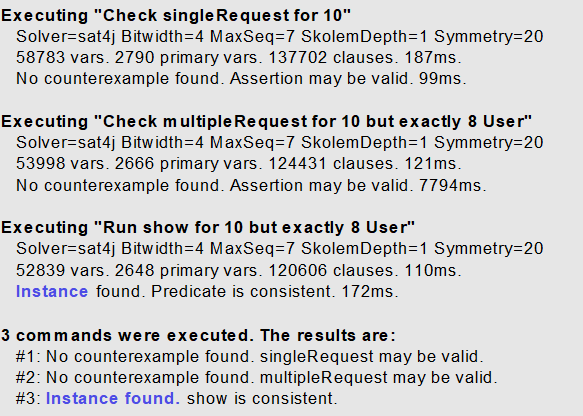
\includegraphics[scale=0.70]{pictures/Results_D4H.png}}
        \caption{ }
        \label{ fig:D4H-Results }
    \end{figure}
    
    \begin{figure}[H]
        \centering
        \makebox[\textwidth][c]{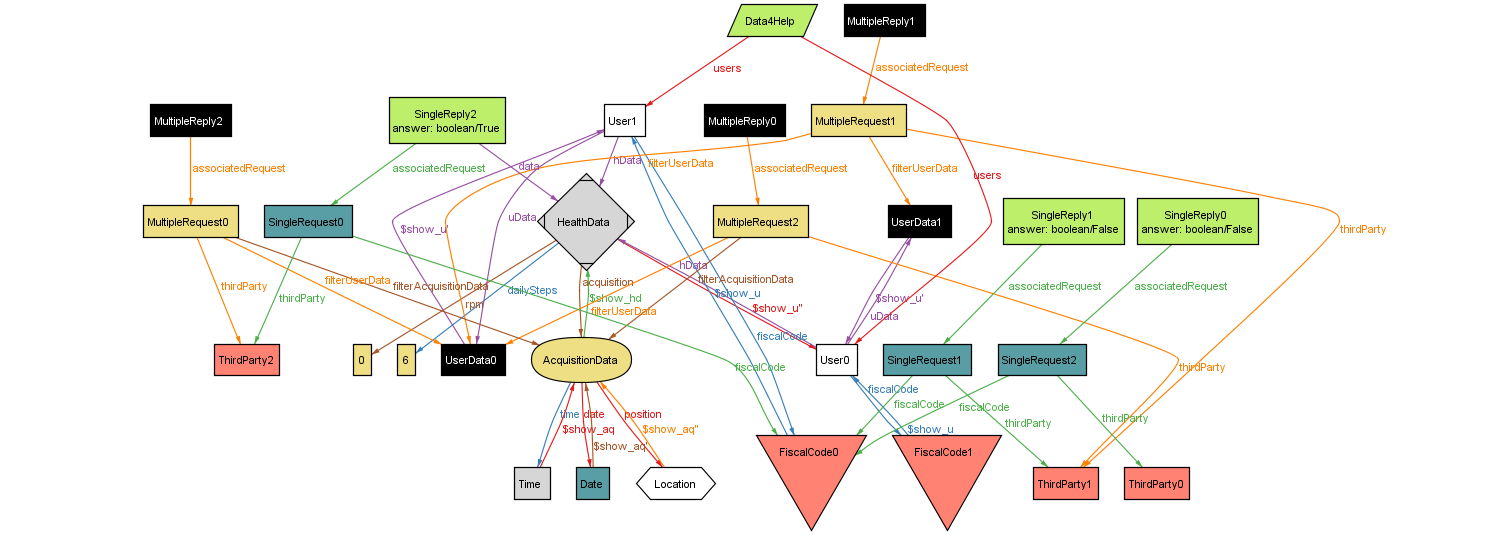
\includegraphics[scale=0.40]{pictures/modelD4H_SingleOk&Not.png}}
        \caption{ }
        \label{ fig:D4H-single-model }
    \end{figure}
    
    \begin{figure}[H]
        \centering
        \makebox[\textwidth][c]{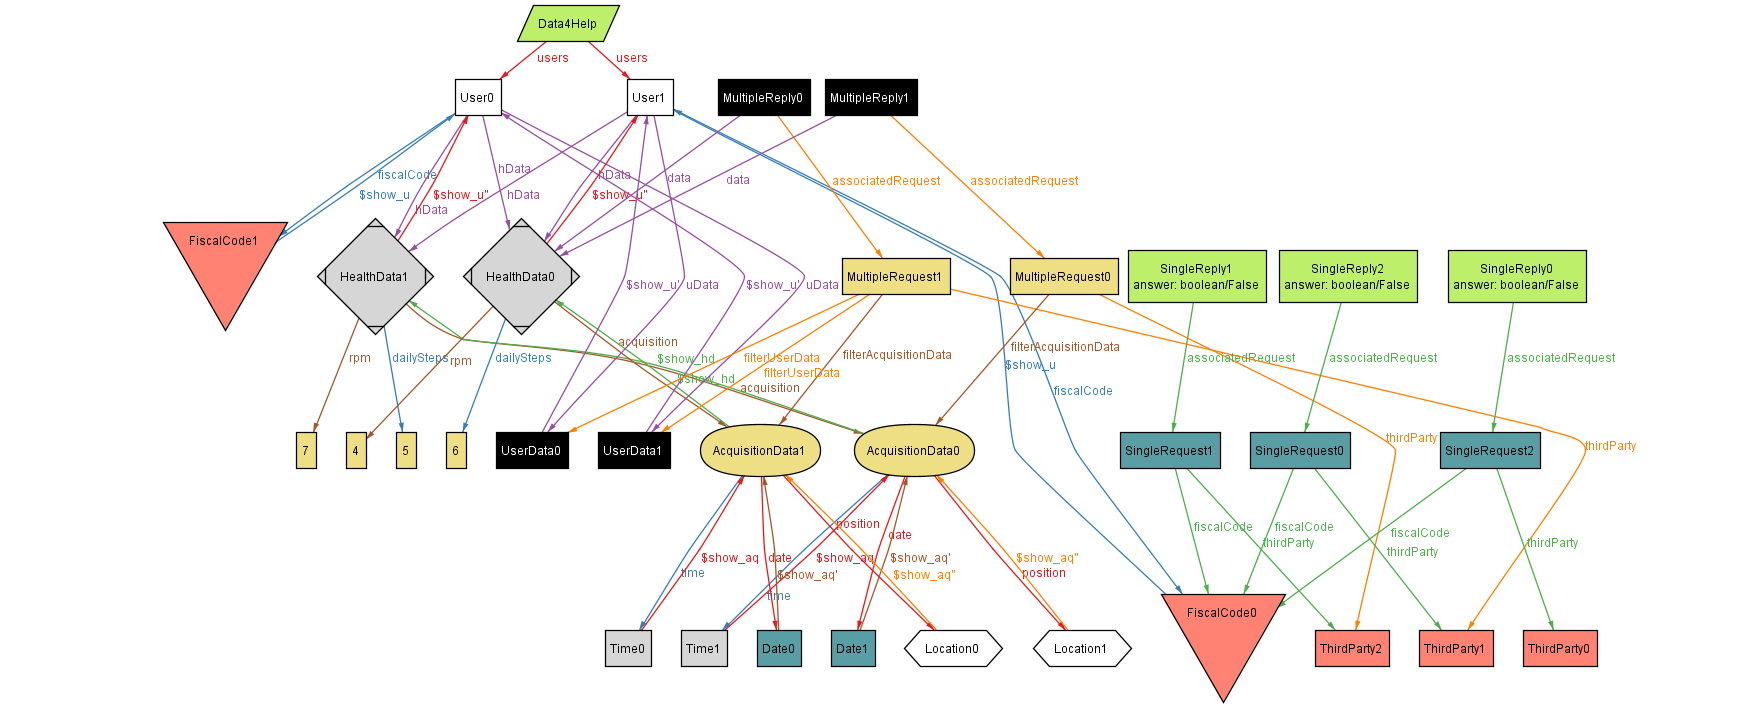
\includegraphics[scale=0.35]{pictures/modelD4H_MulReqOk.png}}
        \caption{ }
        \label{ fig:D4H-multiple-model }
    \end{figure}

    \subsection{AutomatedSOS results}
    On the other hand, the predicates above verify if the model of AutomatedSOS respect the constraint. Therefore, it proves the presence of an ambulance request if and only if a registered user has an hearth frequency too high or too low in relation to some thresholds.\\
    
\begin{lstlisting}[language=alloy]
    check ambulanceRequestWhenBpmNotOutOfBound for 10
    check noAmbulanceWhenBpmOutOfBound for 10
    run show for 10
\end{lstlisting}

    \begin{figure}[H]
        \centering
        \makebox[\textwidth][c]{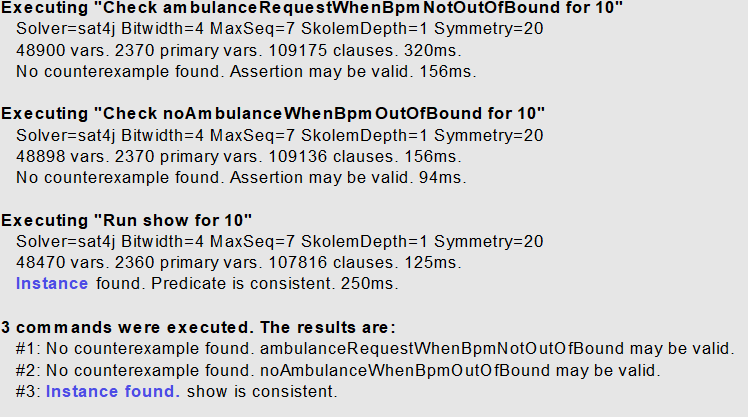
\includegraphics[scale=0.70]{pictures/Results_ASOS.png}}
        \caption{ }
        \label{ fig:ASOS-Results }
    \end{figure}
    
    \begin{figure}[H]
        \centering
        \makebox[\textwidth][c]{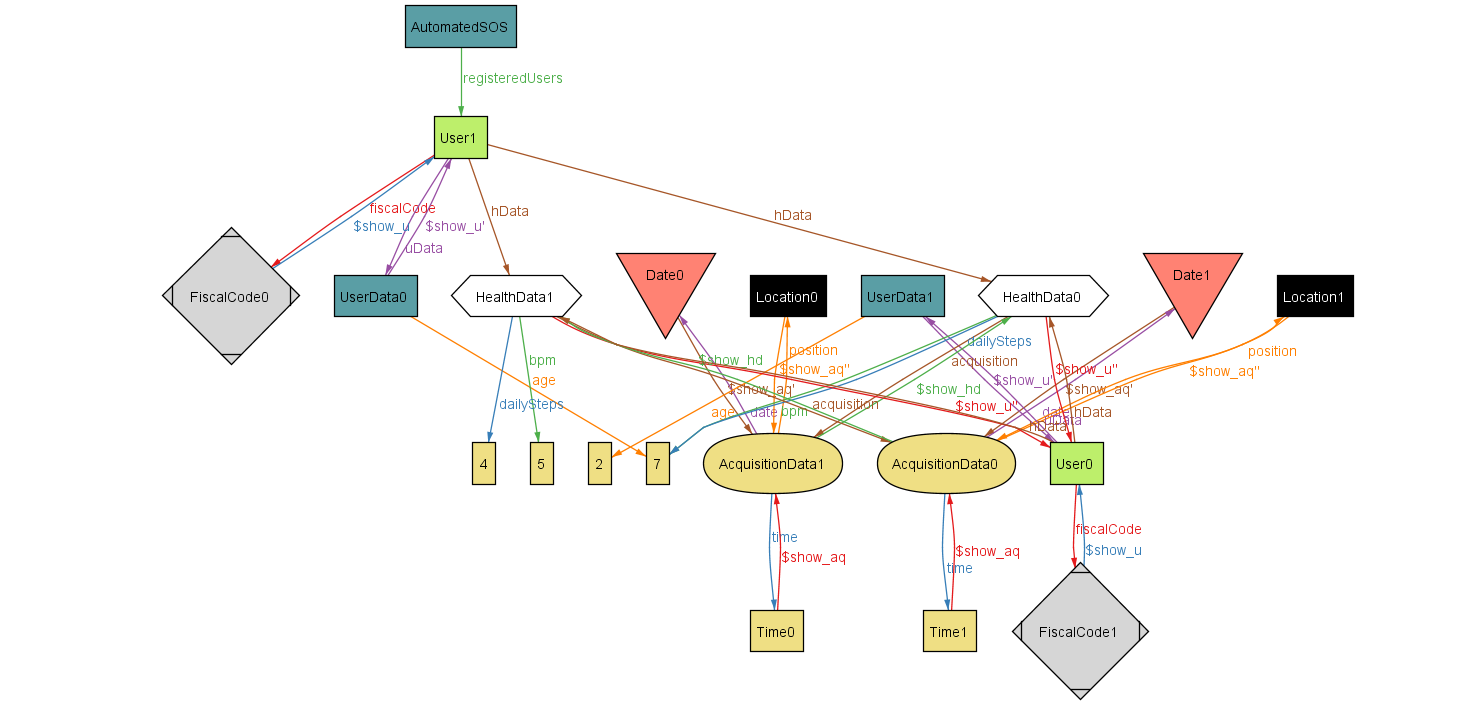
\includegraphics[scale=0.40]{pictures/modelASOS_caseOfBpmOK.png}}
        \caption{ }
        \label{ fig:ASOS-model-bpm-ok }
    \end{figure}
    
    \begin{figure}[H]
        \centering
        \makebox[\textwidth][c]{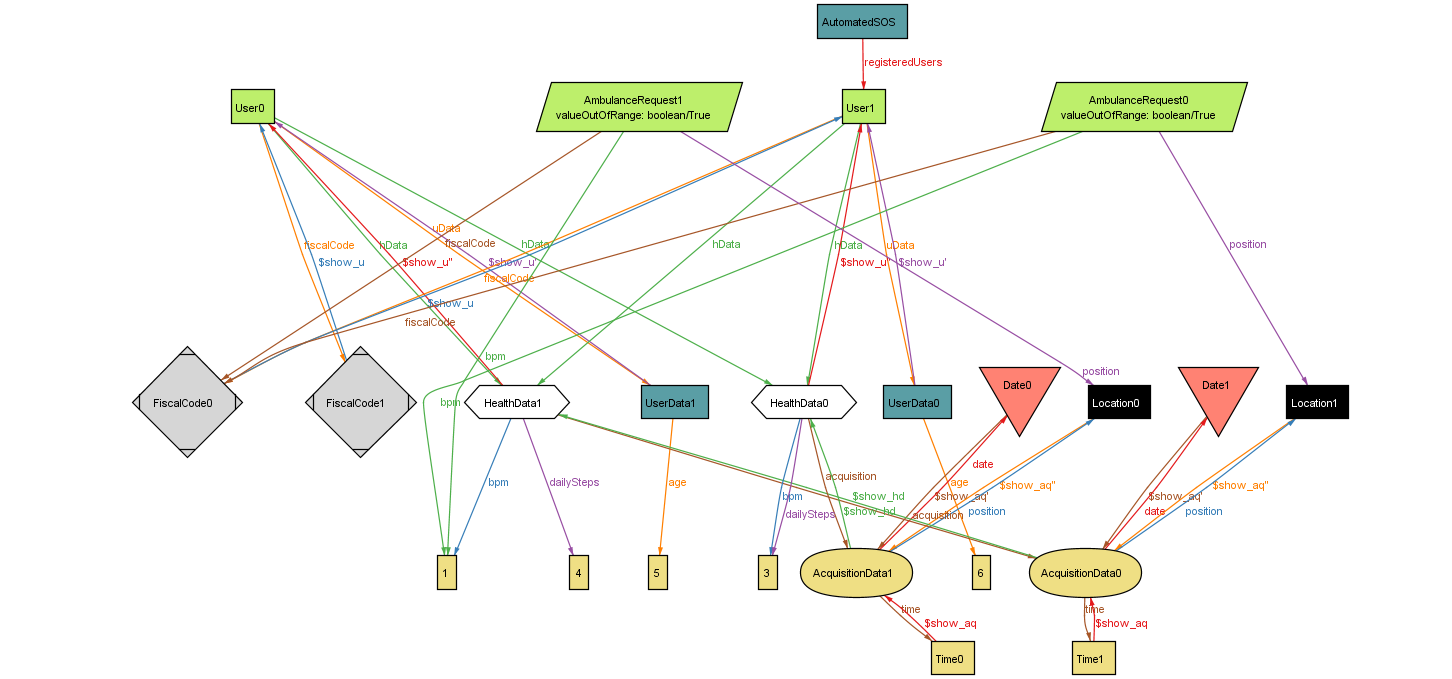
\includegraphics[scale=0.40]{pictures/modelASOS_caseRequest.png}}
        \caption{ }
        \label{ fig:ASOS-model-request }
    \end{figure}

    \subsection{Track4Run results}
    In the last service, Track4Run, the predicate verifies that a visitor can track only the participants enrolled to the race followed by him.
   
\begin{lstlisting}[language=alloy]
    check noVisitorLookingToParticipantsOfDifferentRace for 10
    run show for 10
\end{lstlisting} 
    
    \begin{figure}[H]
        \centering
        \makebox[\textwidth][c]{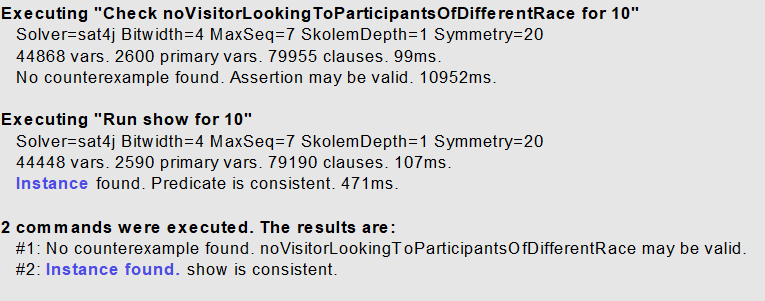
\includegraphics[scale=0.70]{pictures/Results_T4R.png}}
        \caption{ }
        \label{ fig:T4R-Results }
    \end{figure}
    
    \begin{figure}[H]
        \centering
        \makebox[\textwidth][c]{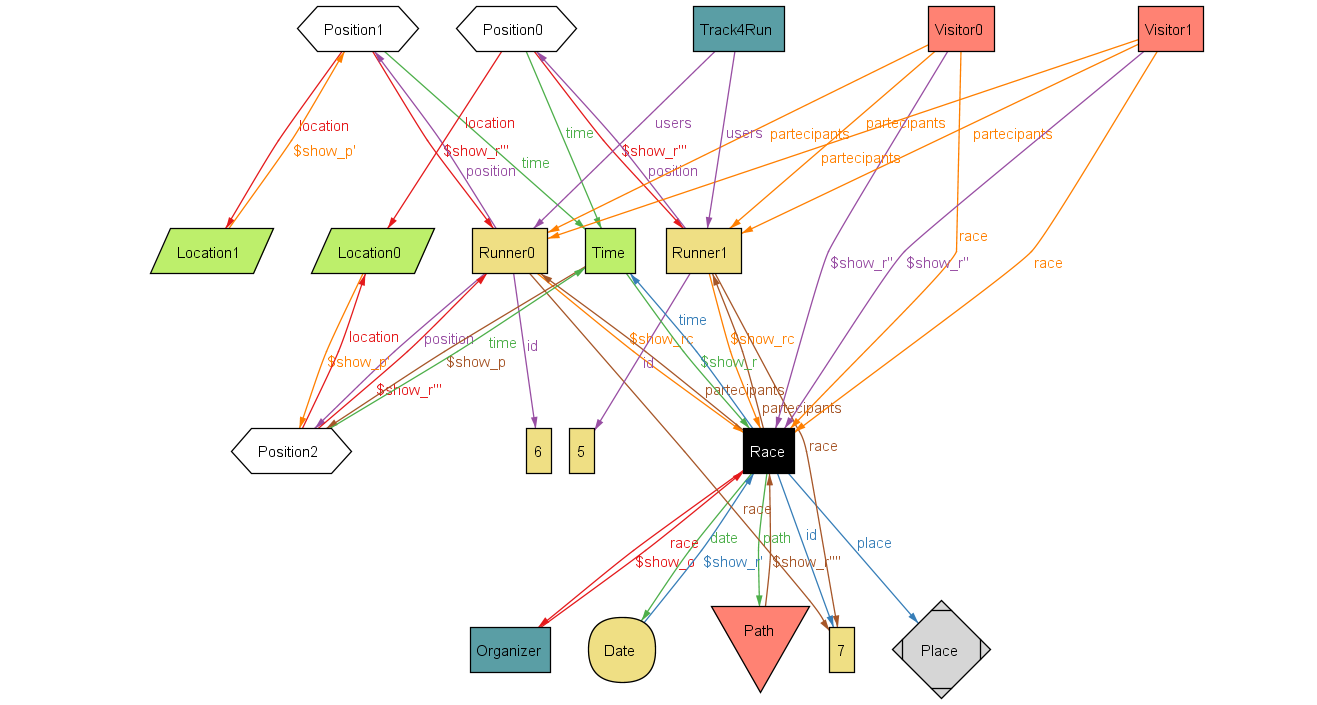
\includegraphics[scale=0.40]{pictures/modelT4R.png}}
        \caption{ }
        \label{ fig:T4R-model }
    \end{figure}
    
    The following pictures shows the result of each predicates and a model represents through a simplified graph.
